\begin{frame}[label=opening]{Darcy Problem}
    \frametitle{Opening}
    \framesubtitle{Darcy Problem}
    \begin{columns}[T]
        \begin{column}{.5\textwidth}
            \only<1>{
                \begin{figure}
                    \centering
                    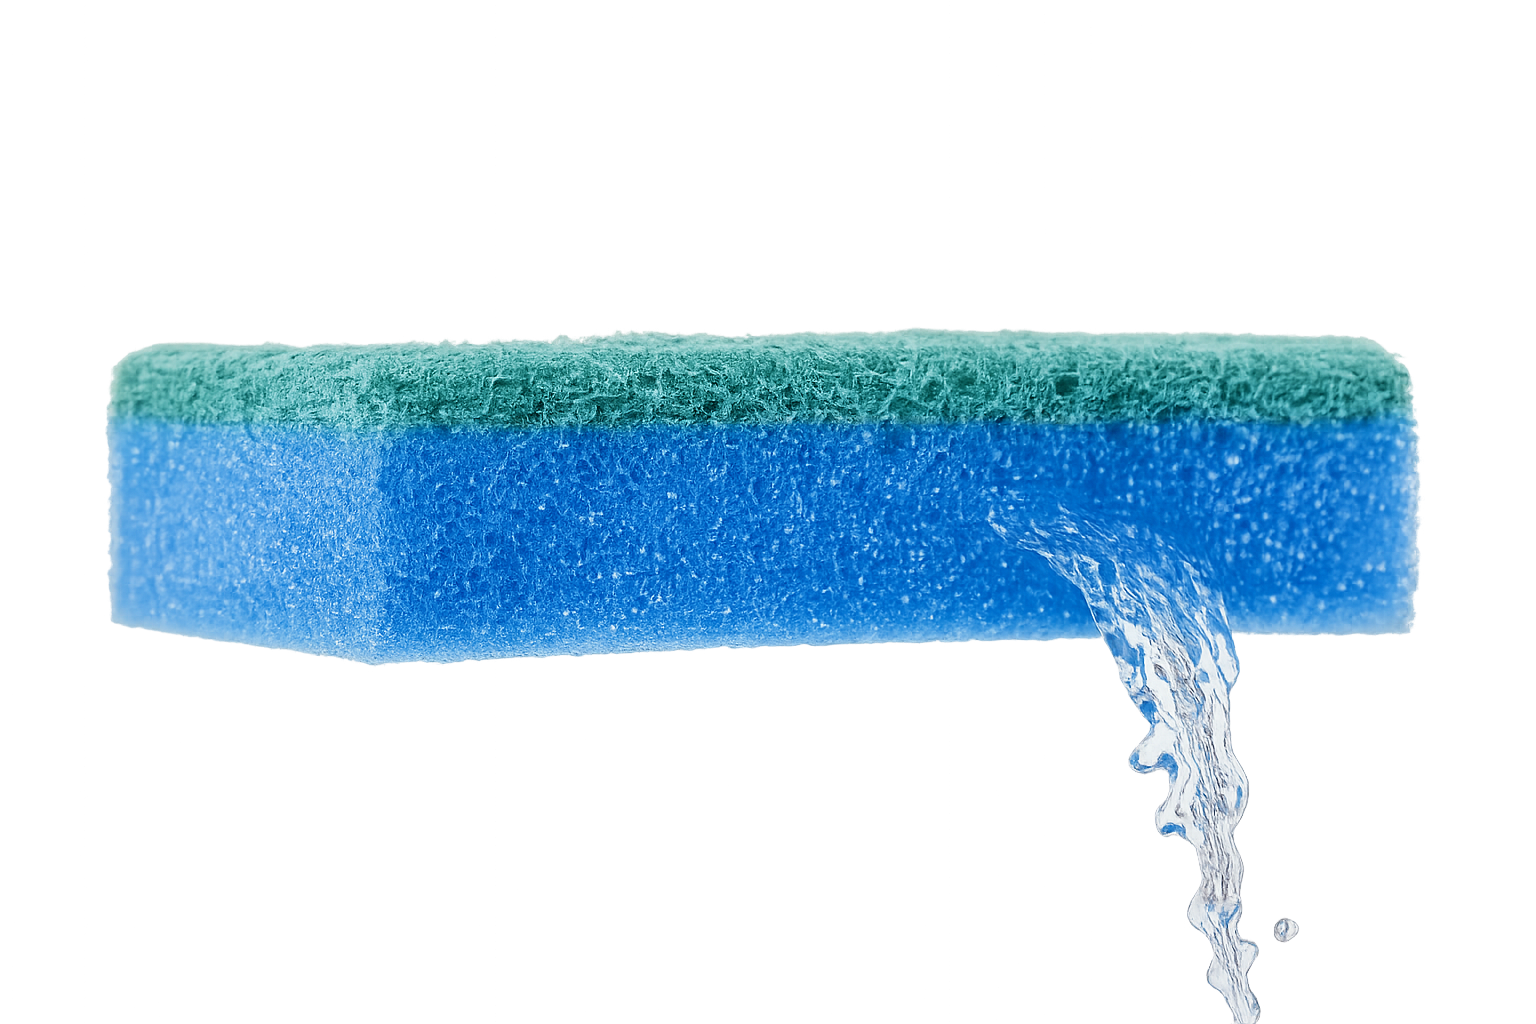
\includegraphics[width=\textwidth]{sponge.png}
                \end{figure}
            }
            \only<2-3>{
                \begin{figure}
                    \centering
                    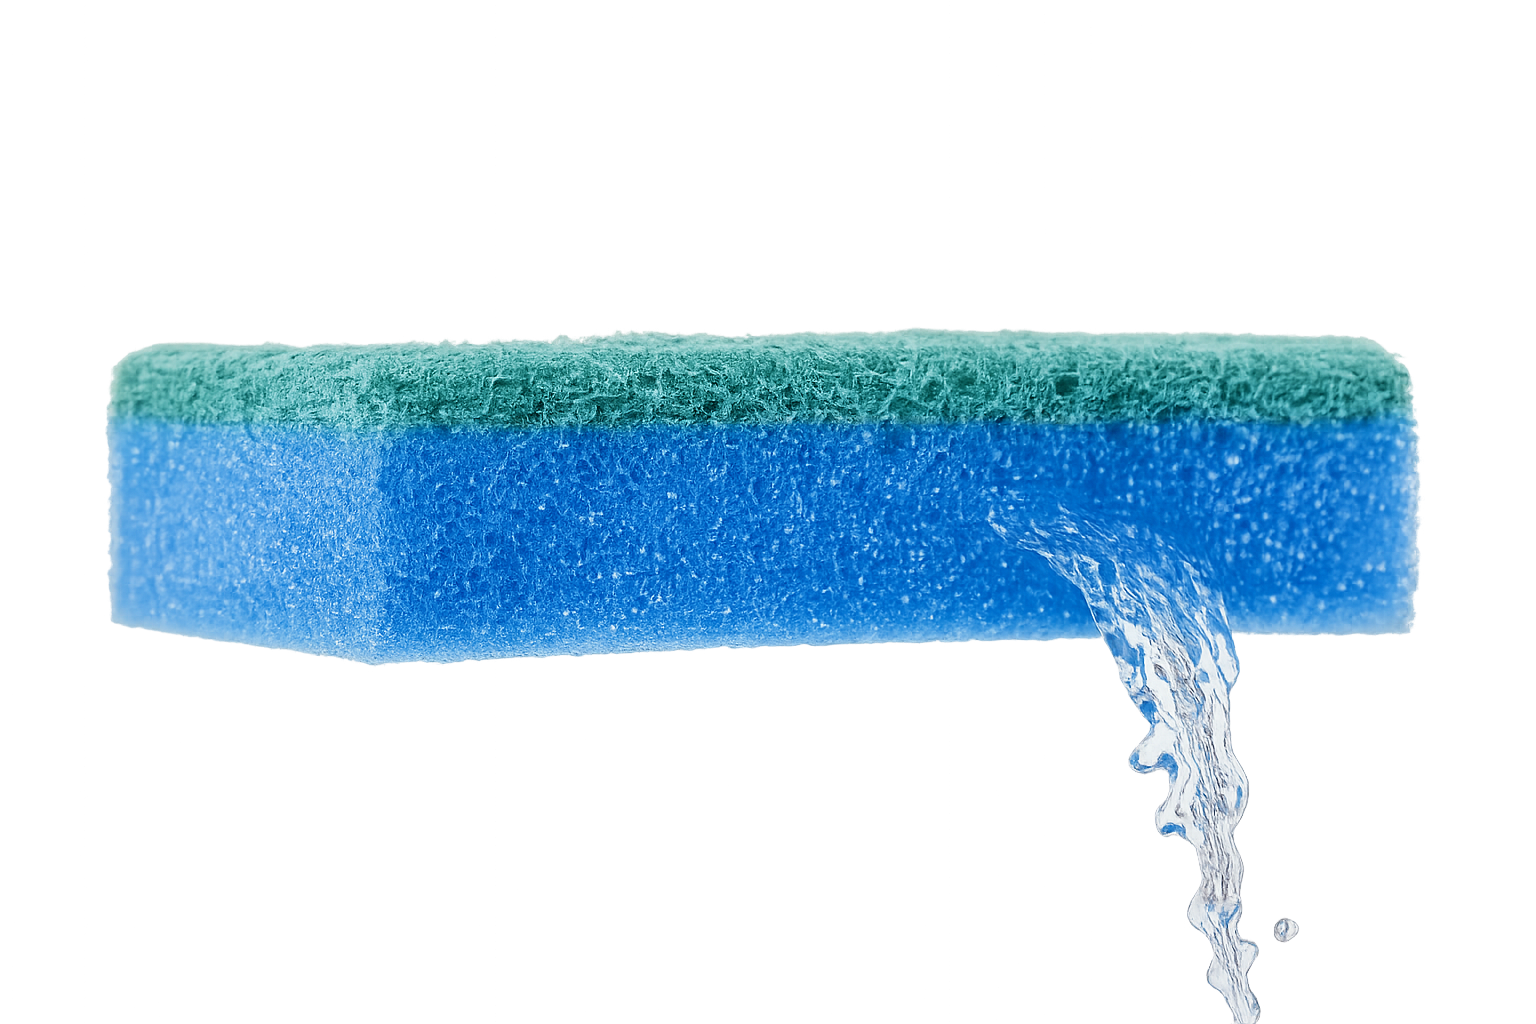
\includegraphics[width=\textwidth]{sponge_water.png}
                \end{figure}
            }
        \end{column}
        \begin{column}{.5\textwidth}
            \only<3>{
                \begin{figure}
                    \centering
                    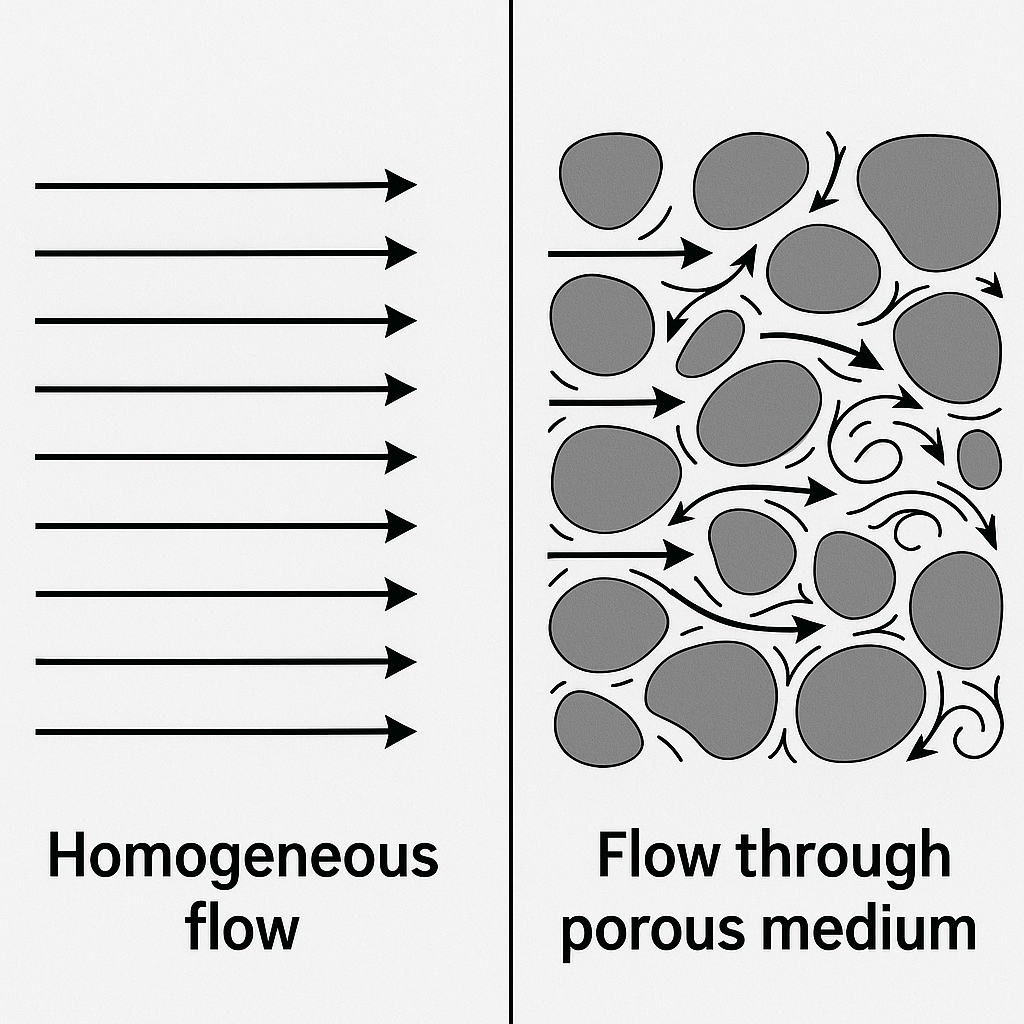
\includegraphics[width=0.8\textwidth]{homogeneous_vs_heterogeneous_flow.png}
                \end{figure}
            }
        \end{column}
    \end{columns}
    \only<4->{
        \begin{itemize}
            \item<4-> Simpler case; high-contrast diffusion problem for $u, u_D \in H^1(\Omega)$, $f\in L^2(\Omega)$ and $\mathcal{C}\in L^{\infty}(\Omega)$
                \begin{equation*}
                    \begin{aligned}
                        -\nabla\cdot\left(\mathcal{C}\nabla u\right) & = f \quad \text{in } \Omega           \\
                        u                                            & = u_D \quad \text{on } \partial\Omega
                    \end{aligned}
                \end{equation*}
            \item<5-> Find $u \in V = \{u\in H^1(\Omega) | u_{\delta \Omega} = u_D\}$
                \begin{equation*}
                    a(u, w) = \int_\Omega \mathcal{C}\nabla u\cdot\nabla w\,dx = \int_\Omega f w\,dx = (f, w) \quad \text{for all } w\in H^1_0(\Omega).
                \end{equation*}
            \item<6-> Introduce some computational mesh $\mathcal{T}_h$ with DOFs $\mathcal{N}$
            \item<7-> Discretize $V_h\subset V$ and $V_{h,0} = V_h \cap H^1_0(\Omega) = \text{span}\{\phi_k\}_{\in\mathcal{N}}$
                \begin{equation*}
                    A\mathbf{u} = \mathbf{b} \quad A_{ij} = a(\phi_j, \phi_i)_{L^2} \quad b_i = (f, \phi_i) \quad \forall i,j\in\mathcal{N}
                \end{equation*}
        \end{itemize}
    }
\end{frame}